%\section*{Summary}
%
%\begin{itemize}
%\item SPDHG excellent alg for non-smooth priors, but only sinogram
%\item modern TOF PET data is extremly sparse (Figure) -> SPDHG inefficient
%      in terms of memory and speed
%\item LM projections are much faster than sino projections for usual count levels
%      (Table)
%\item propose LM-SPDHG that solves both issues
%\item 1st step: better init
%\item 2nd step: rewrite SPDHG in terms of LM updates
%\end{itemize}

%%%%%%%%%%%%%%%%%%%%%%%%%%%%%%%%%%%%%%%%%%%%%%%%%%%%%%%%%%%%%%%%%%%%%%%%%%%%%%%%%%%%%%%%%%%%%%%%%%%%%%%%
%%%%%%%%%%%%%%%%%%%%%%%%%%%%%%%%%%%%%%%%%%%%%%%%%%%%%%%%%%%%%%%%%%%%%%%%%%%%%%%%%%%%%%%%%%%%%%%%%%%%%%%%
%%%%%%%%%%%%%%%%%%%%%%%%%%%%%%%%%%%%%%%%%%%%%%%%%%%%%%%%%%%%%%%%%%%%%%%%%%%%%%%%%%%%%%%%%%%%%%%%%%%%%%%%
%%%%%%%%%%%%%%%%%%%%%%%%%%%%%%%%%%%%%%%%%%%%%%%%%%%%%%%%%%%%%%%%%%%%%%%%%%%%%%%%%%%%%%%%%%%%%%%%%%%%%%%%

\section{Introduction}

A major challenges of image reconstruction in positron emission tomography (PET)
is noise suppression since the acquired emission data suffer from high levels of Poisson
noise due to limitations in acquisition time, injectable dose and scanner sensitivity.
To limit the transfer of the data noise into the image during model-based iterative
reconstruction (MBIR), different strategies exist. 
One possibility is to add a ``smoothing'' prior to the data fidelity term in the cost
function that is being optimized.
In general, we can write the optimization problem for PET image reconstruction as
%
\begin{equation}
\argmin _{x\geq 0} \sum_{i=1}^{m} \underbrace{(Px + s)_i -  d_i \log \left( (Px + s)_i \right)}_{D_i(x)} + \, \beta R(Kx),
\label{eq:primal}
\end{equation}
%
where $x$ is the PET image to be reconstructed, $P$ is the (TOF) forward model including the effects
of attenuation and normalization and blurring, $d$ are the acquired prompt TOF coincidences 
(the emission sinogram), and $s$ are additive contaminations including random and 
scattered coincidences. 
$\sum_{i=1}^m D_i(x)$ is the negative Poisson log-likelihood, $i$ is the index of the data (TOF sinogram)bin and $m$ is the total number of data (TOF sinogram) bins.
$R(Kx)$ is the ``smoothing prior'' consisting of a generic linear operator $K$ that calculates 
local differences and a proper, convex, lower-semicontinous function $R$.
The level of regularization is controlled by the non-negative scalar factor $\beta$.
A specific example for $K$ would be the gradient operator $\nabla$, e.g. approximated by finite forward 
differences in the discretized setting.
Using the gradient operator for $K$ and the mixed L2-L1 norm for $R$ leads to the well-known 
Total Variation (TV) prior \cite{Rudin1992}.

Unfortunately, many advanced smoothing priors aiming for edge-preservation 
such as e.g. TV \cite{Rudin1992}, Total Generalized Variation (TGV) 
\cite{Bredies2010}, Joint T(G)V \cite{Rigie2015,Knoll2016}
Parallel Level Sets \cite{Ehrhardt2016a,Schramm2017} or directional Total Variation (DTV)
\cite{Ehrhardt2016} use non-smmoth functions for $R$ which permits the use of simple and efficient 
purely gradient-based optimization algorithms to solve \eqref{eq:primal}.

\subsection*{PDHG and SPDHG for PET reconstruction}

Using the fact that $D(x) = \sum_i D_i(x)$ and $R(x)$ are equal to their convex biconjugates 
$D^{**}(x) = \sup_y \langle Px + s, y \rangle - \sum_{i=1}^{m} D_i^*(y_i)$ 
and $R^{**}(x) = \sup_w \langle Kx, w \rangle - R^*(w)$, respectively, and that 
$(\beta R(x))^* = \beta R^*(w / \beta)$, we can rewrite \eqref{eq:primal} as the saddle point problem
%
\begin{equation}
\argmin _{x\geq 0} \, \sup_{y,w} \,  \langle Px + s, y \rangle + \langle Kx, w \rangle - \sum_{i=1}^{m} D_i^*(y_i) - \beta R^*(w/\beta) ,
\label{eq:saddle}
\end{equation}
%
introducing the dual variables $y$ and $w$ and the convex dual of the Poisson log-likelihood given by
%
\begin{equation}
D_i^*(y_i) =
\begin{cases}
-d_i + d_i \log \left( \frac{d_i}{1-y_i} \right) & \text{if } y_i < 1 \\
\infty & \text{else} \ .
\end{cases}
\end{equation}
%
Problem \eqref{eq:saddle}, can be solved using the generic primal-dual hybrid gradient (PDHG) 
algorithm by Chambolle and Pock \cite{Chambolle2011} even for non-smooth priors.
PDHG is in iterative algorithm that requires the evaluation of the complete forward and adjoint operator
in every update.
The usage of the original PDHG algorithm to solve \eqref{eq:saddle} for real-world state-of-the-art
TOF PET systems usually means extremly long computation times, because evaluation of $P$ (corrected TOF 
forward projection) and $P^T$ (corrected TOF back projection) 
for state-of-the-art TOF PET systems are usually slow and because several hundreds to thousand of updatesare needed to obtain reasonable convergence.

To overcome this limitatation, Chambolle et al. published a stochastic extension of PDHG called SPDHG 
for saddle point problems that are separable in the dual variable \cite{Chambolle2018} in 2018.
In contrast to PDHG, SPDHG has the advantage that the complete forward and adjoint operator is 
split into $n$ subsets and that in every update only a random subset of the forward
and adjoint operator chosen according to probability $p_k$ have to be evaluated.
In \cite{Ehrhardt2019}, Ehrhardt et al. applied SPDHG to 3D non-TOF PET reconstruction with TV-like
priors and could indeed show that around 10 complete projections and back projections are sufficient 
to obtain reasonable convergence using SPDHG with 252 subsets.
Moreover, the authors also demonstrated that preconditioning further accelerates convergence.
The resulting SPDHG algorithm to solve \eqref{eq:saddle} is summarized in Algorithm \ref{alg:spdhg},
where the proximal operator of the convex conjugate of the negative Poisson log-likehood $D_i^*$ 
can be calculated point-wise and is given by
%
\begin{equation}
\begin{split}
(\prox_{D_i^*}^{S}(y))_i &= \prox_{D_i^*}^{S}(y_i) \\ 
&= \frac{1}{2} \left(y_i + 1 - \sqrt{ (y_i-1)^2 + 4 S_i d_i} \right) \ .
\end{split}
\label{eq:proxD}
\end{equation} 
%
The proximal operator for $R^*$, obviously depends on choice of $R$ but can be also efficiently 
computed using point-wise operations for many popular choices of $R$.
As mentioned in \cite{Ehrhardt2019}, Algorithm \ref{alg:spdhg} converges if we use the preconditioned
step sizes
%
\[ S_k = \gamma \, \text{diag}(\frac{\rho}{P_k 1} )\qquad  T_k = \gamma^{-1} \text{diag}(\frac{\rho p_k}{P^T_k 1}) \ , \]
% 
and
%
\[ S_{n+1} = \gamma \, \frac{\rho}{\|K\|} \qquad T_{n+1} = \gamma^{-1} \frac{p_i\rho}{\|K\|} \ , \]
%
setting $T = \min_{k=1,\ldots,n+1} T_i$ pointwise, and choosing $\rho<1$ and $\gamma>0$.
%
\begin{algorithm}[t]
\begin{algorithmic}[1]
\small
\State \textbf{Initialize} $x(=0),y(=0),(w=0)$, $(S_i)_i,T,(p_i)_i$,
\State $\overline{z} = z = P^T y + K^T w$
\Repeat
	\State $x = \proj_{\geq 0} (x - T \overline{z})$
	\State Select $i \in \{ 1,\ldots,n+1\} $ randomly according to $(p_i)_i$
  \If{$i \leq n$}
	\State $y_i^+ \gets \prox_{D_i^*}^{S_i} ( y_i + S_i  ( P_i x + s_i))$
	\State $\delta z \gets P_i^T (y_i^+ - y_i)$
	\State $y_i \gets y_i^+$
  \Else
	\State $w^+ \gets \beta \prox_{R^*}^{S_i/\beta} ((w + S_i  K x)/\beta)$
	\State $\delta z \gets K^T (w^+ - w)$
	\State $w \gets w^+$
  \EndIf
	\State $z \gets z + \delta z$
	\State $\overline{z} \gets  z + (\delta z/p_i)$
\Until{stopping criterion fulfilled}
\State \Return{$x$}
%\EndFunction
\end{algorithmic}
\caption{SPDHG for PET reconstruction \cite{Ehrhardt2019}}
\label{alg:spdhg}
\end{algorithm}
%

\subsection*{Limitations of PDHG and SPDHG for PET reconstruction}

Whilst SPDHG is a big step forward for an efficient solution of \eqref{eq:saddle} using
in terms of computational speed, it also comes with two main limitations.
First of all, as discussed in Remark 2 of \cite{Ehrhardt2019}, 
a potential drawback of SPDHG is that it requires to keep at least one more complete 
(TOF) sinogram in memory (the dual variable $y$). 
Moreover, if the proposed preconditioning is used, a second complete (TOF) sinogram
(the sequence of step sizes $(S_k)_{k=1}^n$) needs to be stored in memory.
The latter is not a major problem for static single-bed non-TOF PET data, where sinogram sizes
are relatively small.
However, for simultaneous multi-bed, dynamic or TOF PET data, the size of the complete data sinograms
can be become problematic, especially when we would like to run Algorithm \ref{alg:spdhg} on
state-of-the-art GPUs with limited memory.
E.g., for a TOF PET scanner with 25\,cm axial FOV and a TOF resolution of ca. 400\,ps, 
a complete unmashed static TOF sinogram for one bed position 
has approximately $4.4\cdot10^9$ data bins, requiring ca. 17\,GB of memory in 32\,bit floating
point precision.
Note that with improved TOF resolution and increasing axial field of view (e.g. total body 
PET scanners), the memory required to store a complete TOF sinogram will substantially increase
in the future.

Second, PDHG and SPDHG only work with ``binned'' data.
In the case of TOF PET reconstruction that means that the acquired raw listmode data first needs to be
binned into TOF sinograms and that the forward and back projections need to be computed using
sinogram projectors.
For most acquisitions with modern TOF PET scanners, this is inefiicient both in terms of memory and
computational time since the TOF emission data is extremely sparse.
In contrast, storage and processing of the data in listmode format (event by event) is usually 
more efficient.

\subsection*{Sparsity of TOF PET data}

In contrast to non-TOF PET emission sinograms, TOF PET emission sinograms of most acquisitions
with state-of-the-art TOF PET scanners are extremely sparse.
This is because the every geometrical line of response (LOR) has to be subdivided into
several small TOF bins.
To achieve sufficient sampling of the TOF information, the number of TOF bins has to
inversely propotional to the TOF resolution of the scanner. 
Consequently, for a fixed number of acquired prompt coincidences, the sparsity of the
sinogram is proportional to the TOF resolution.

As an example, for a typical 80\,s-per-bed-position whole-body FDG scan with an injected dose 
of around 323\,MBq acquired 60\,min p.i. on a state-of-the-art TOF PET/CT scanner with
20\,cm axial FOV, more than 94\% of the data (TOF sinogram) bins are empty.
An example that demonstrates this extreme sparsity of TOF sinograms is shown in Fig.~\ref{fig:sparsity}.
For shorter frames, as present e.g. in the early phase of dynamic scans or when gating is used, 
the fraction of empty bins can even higher.
%And even for ``high count'' late static 20\,min FDG brain scans with an injected dose of 150\,MBq
%acquired 60\,min p.i., still around 70\% of the data bins are empty.

Note that we expect that the sparsity of the TOF emission data of future PET systems will increase 
faster than linear compared to the improvement of the TOF resolution.
This is because with better TOF resolution, every detected event carries more information such
that fewer detected events are needed to reconstruct images with the same variance \cite{Tomitani1981}.

\begin{figure}
  \centering
    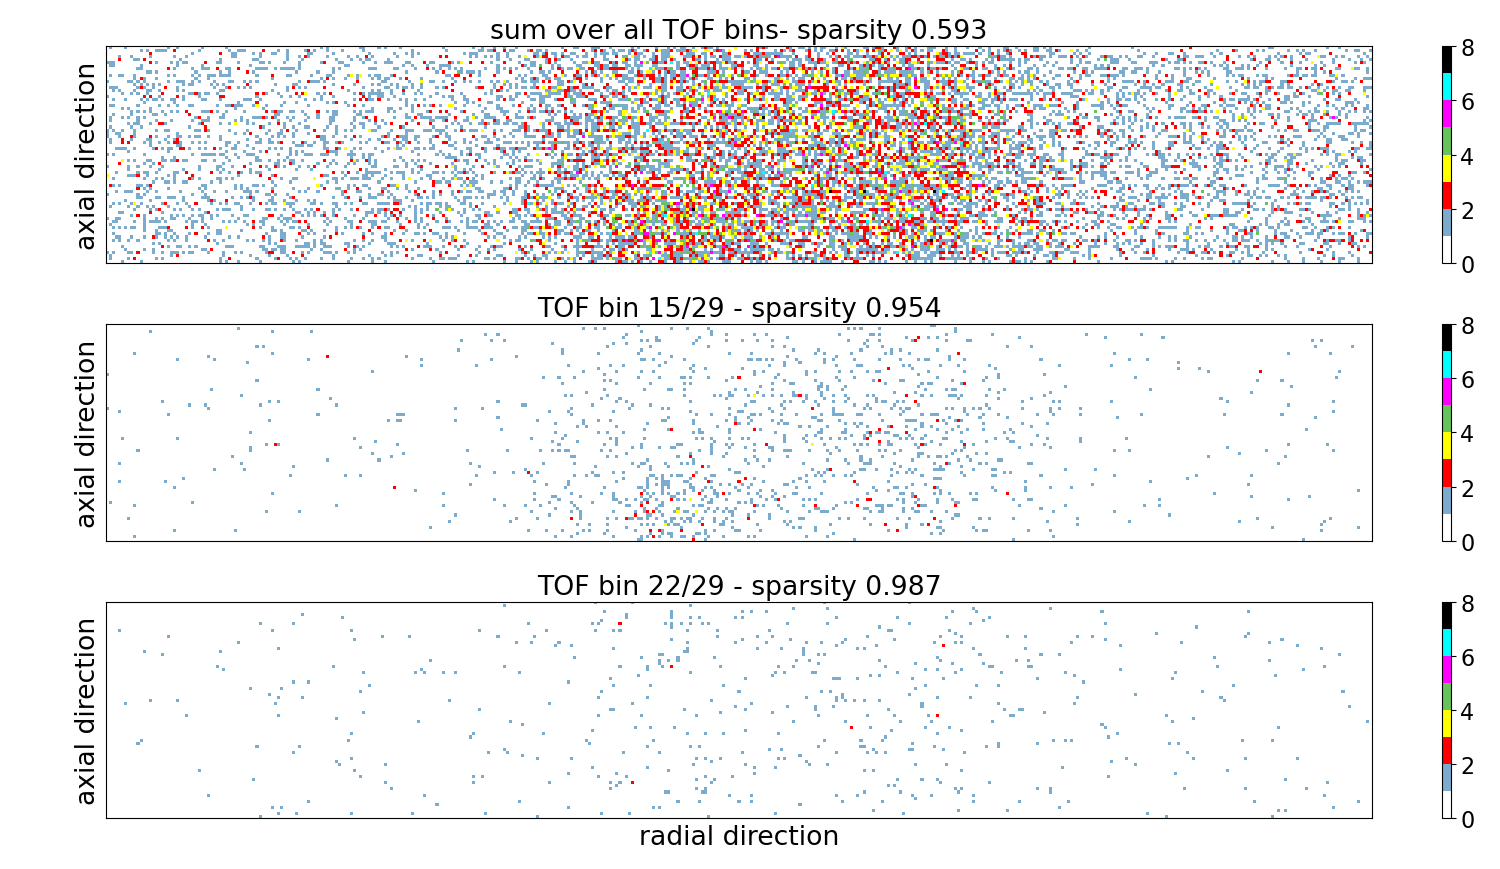
\includegraphics[width=1.0\columnwidth]{./figs/sparsity.png}
  \caption{Representative slices through a single view of an emission sinogram of an 
  80s [\textsuperscript{18}F]FDG acquisition of a liver bed position. 
  The scan was acquired 1\,h post injection with an injected dose of 323\,MBq on
  a GE DMI PET/CT with a TOF resolution of 400\,ps (29 TOF bins). 
  The horizontal and vertical axis represent the radial and axial direction (direct planes only), 
  respectively. 
  (top) sum over all TOF bins. (middle) central TOF bin 15/29 with 94\% empty bins. 
  (bottom) TOF bin 22/29 with 97\% empty bins.}

  \label{fig:sparsity}
\end{figure}


\subsection*{Contributions and Aim}

To improve the efficiency of SPDHG in terms of memory and computation time when reconstructing 
sparse TOF PET data, we propose and analyze a listmode version of the SPDHG algorithm (LM-SPDHG) 
that allows event-by-event processing using dedicated listmode forward and back projectors.
We first of all derive LM-SPDHG from SPDHG and show that the convergence of LM-SPDHG is as 
fast as the convergence of SPDHG based on dedicated numeric examples.
Moreover, we analyze the requirements in terms of memory and computational time
for LM-SPDHG compared to SPDHG for typical scans acquired on state-of-the-art TOF scanners.


\section{Theory and Algorithms}

In the next subsection, we first of all show how to reduce the memory requirements
when reconstructing sparse TOF sinograms before deriving the complete LM-SPDHG algorithm.

\subsection*{Memory-efficient SPDHG for sparse TOF sinograms}

As shown in \cite{Schramm2021}, the memory requirements for SPDHG can substantially reduced by choosing
a better intialization of the dual variable $y$.

From Eq.~(\ref{eq:proxD}) we can observe that for data bins $i$ where $d_i = 0$ 
(empty TOF sinogram bins), $\prox_{D_i^*}(a_i) = 1$ for $a_i \geq 1$ and $\prox_{D_i^*}(a_i) = a_i$ 
otherwise. 
Moreover, we see that $ a_i = y_i + S_i (P_i x + s_i) \geq 1$ provided that $y_i \geq 1$ 
since all other quantities are non-negative. 
Consequently, if we initialize all bins of $y$ where the data $d$ equals zero with one, 
these bins of $y$ remain $1$ during all iterations. 
This in turn means that these bins do not contribute to the update of $\delta z$, $z$, $\bar{z}$, 
and $x$, since only the difference between
$y$ and $y^+$ is backprojected in line 8 of algorithm~\ref{alg:spdhg} and
do not have to be kept in memory during the iteration loop (lines 3 until 17). 
The only place where the empty data bins contribute is the initialization of $z$ and $\bar{z}$
in line 2.
However, this linear one time operation can be split into smaller chunks to also reduce
the required memory of this step.

At a first glance the initialization of $y$ proposed above seems very artificial.
But, if we construct a better initialization $y^0$ in a way such that it is the solution of our
saddle point problem \eqref{eq:saddle} for a fixed initial $x^0$, it has to satisfy
%
\begin{equation}
\langle P x^0, y^0 \rangle - D^*(y^0) = D(Px^0 + s) \ ,
\end{equation}
%
which is the case when
%
\begin{equation}
y^0 \in \partial D(Px + s) |_{x^0} \ .
\end{equation}
%
Since $D$ (the negative Poisson loglikelihood) is differentiable, this leads
to the condition
\begin{equation}
y^0 = 1 - \frac{d}{Px^0 + s} \ ,
\label{eq:yinit}
\end{equation}
where the division is to be understood point-wise.
We see that under this condition, $y^0$ is indeed one in bins where $d$ is zero,
irrespective of the choice of $x^0$.
As argued above, this improved intialization of $y$ naturally reduces the 
memory requirements of SPDHG and also improves the speed of convergence in case a
``warm start'' for $x^0$ is chosen. 
The latter can be e.g. achieved by applying one iteration
and a reasonable amount of subsets of the EM-TV algorithm \cite{Sawatzky2008, Burger2008} 
which can be also implemented in a listmode way. 
Note that EM-TV in general seems to be an appealing algorithm to solve our optimization
problem \eqref{eq:primal} also for data in listmode format.
However, in contrast to SPDHG, EM-TV does not converge when using subsets, as will
be shown later.

\subsection*{Listmode SPDHG}

As indicated by the name, emission data in listmode format are a chronological list $N$ of detected 
events $e \in N$, where each event is characterized by a small set of numbers 
(e.g. the number of the two detectors, the discretized TOF difference, and a time stamp).
To process the listmode data during reconstruction without binning it into a sinogram,
we introduce the listmode forward operator $P_N$ mapping the image data $x$ to a 
data-vector of dimension $|N|$ via \[ (P^{LM}_N x)_e  = (Px)_{i_e} , \text{ for each }e \in N,\]
where $i_e$ is the sinogram bin in which event $e$ was detected.

Re-writing the gradient of the negative Poisson loglikihood using listmode data and the
listmode operators is straight forward such that any gradient-based
PET reconstruction algorithm can be easily adapted to listmode data.
However, for SPDHG - which has the advantage of being able to handle non-smooth priors and
has guaranteed convergence, an adaptation to listmode is possible but more challenging.

\begin{algorithm}[t]
\begin{algorithmic}[1]
\small
\State \textbf{Input} event list $N$, contamination list $s_N$
\State \textbf{Calculate} event counts $\mu_e$ for each e in $N$ (see text)
\State \textbf{Initialize} $x,w,(S_i)_i,T,(p_i)_i$
\State \textbf{Initialize} list $y_{N} = 1 - (\mu_N /(P^{LM}_{N} x + s_{N}))$ 
\State \textbf{Preprocessing} $\overline{z} = z = {P^T} 1 - {P^{LM}}^T (y_N-1)/\mu_N + K^T w$ %(see \eqref{eq:zinit_lm} and text)
\State \textbf{Split} lists $N$, $s_N$ and $y_N$ into $n$ sublists $N_i$, $y_{N_i}$ and $s_{N_i}$
\Repeat
	\State $x = \proj_{\geq 0} (x - T \overline{z})$
	\State Select $i \in \{1,\ldots,n+1\}$ randomly accord. to $(p_i)_i$
  \If{$i \leq n$}
	  \State $y_{N_i}^+ \gets \prox_{D^*}^{S_i} \left( y_{N_i} + S_i \left(P^{LM}_{N_i} x + s_{N_i} \right) \right)$
	  \State $\delta z \gets {P^{LM}_{N_i}}^T \left(\frac{y_{N_i}^+ - y_{N_i}}{\mu_{N_i}}\right)$
	  \State $y_{N_i} \gets y_{N_i}^+$
  \Else
	  \State $w^+ \gets \beta \prox_{R^*}^{S_i/\beta} ((w + S_i  K x)/\beta)$
	  \State $\delta z \gets K^T \left(w^+ - w\right)$
	  \State $w \gets w^+$
  \EndIf
	\State $z \gets z + \delta z$
	\State $\overline{z} \gets  z + (\delta z/p_i)$
\Until{stopping criterion fulfilled}
\State \Return{$x$}
%\EndFunction
\end{algorithmic}
\caption{LM-SPDHG for PET reconstruction}
\label{alg:lmspdhg}
\end{algorithm}


Our proposed listmode SPDHG algorithm (LM-SPDHG) is shown in algorithm~\ref{alg:lmspdhg} and
overcomes those challenges.
In contrast to the original SPDHG using binned data (sinograms), the forward and adjoint
PET models have been replaced by their listmode equivilants as defined above (lines 11 and 12).
Moreover, the dual variable for data fidelity is replaced by the list $y_N$ which has the
same length as the measured event list $N$.
If an event with a fixed sinogram bin $i_e$ occurs more than once in the event list
$N$, it is also forward and back-projected multiple times in steps 11 and 12.
To compensate for this fact, we have to divide by the event count $\mu_e$ before back projection
in line 12.
Note that (i) as shown in Fig.~\ref{fig:sparsity} in most standard acquisitions the event count
of most events is 1 and that (ii) calculating the event count $\mu_e$ which is a pre-requisit
creates a small pre-processing overhead (step 2).
However, when implemented on a modern GPU this overhead is small compared to the computation
time needed to calculate all iterations.
Moreover, it is in the similar order of the time needed to unlist the native listmode data into
a sinogram which is a pre-requisit and pre-processing overhead for SPDHG.

Another difference of LM-SPDHG compared to SPDHG is the fact that we split the data into $n$ subsets by
assigning every $n$-th event of the complete event list $N$ into the $n$-th sub list - 
as commonly done in listmode OSEM.
In that way, we can think of the subset listmode forward operator $P^{LM}_{N_i}$
as the full forward operator $P$ with a sensivity reduced by a factor of $n$.
Accordingly, we set the step sizes associated with the subset listmode PET operators to
%
\begin{equation}
S_k = \gamma \, \text{diag}(\frac{\rho}{P^{LM}_{N_k} 1} )\qquad  T_k = n\,\gamma^{-1} \text{diag}(\frac{\rho p_k}{P^T 1}) \ . 
\label{eq:lm_stepsizes}
\end{equation}
% 
At a first glance, the initialization of $z$ and $\bar{z}$ might look odd.
However, the first part of the expression in step 4 of the LM-SPDHG algorithm equivalent to 
applying the adjoint sinogram operator $P^T$ to a sinogram initialized according to \eqref{eq:yinit}.
Note that step 4 still requires to calcuate a sinogram back projection of a unity sinogram ($P^T 1$)
which, in general, we would like to avoid in listmode data processing.
Unfortunately avoiding this single sinogram backprojection is not possible.
But we note that this ``sensitivity image`` is also needed in the calculation of the step sizes
$T_k$ and also in the listmode EM-TV algorithm that we use to initialize $x$.
Hence, we recommend to pre-compute to sensitivity image ($P^T 1$) and to store it in memory.

In summary, compared to SPDHG, LM-SPDHG as shown in algorithm~\ref{alg:lmspdhg} has the advantage
that (i) only lists ($N$, $y_{N}$, $s_N$, $\mu_N$) instead of complete sinograms 
($y$ and $d$) have to be 
stored in memory and (ii) all projections and back projection can be performed using listmode
projectors.
This means that for all acquisitions where the number of detected events is smaller than
the number of data bins, the required memory and computation time is reduced.
The latter depends on the actual implementation of the sinogram and listmode projectors
and on the computational hardware.
According to our experience using a state-of-the art GPU implementation of a Joseph TOF projectors
for a TOF PET scanner with 400\,ps TOF resolution and 25\,cm axial field of view,
a forward and back projection is faster in listmode if approximately less than 3e8 events 
have to be processed.
For 7e7 and 1e7 counts, the projections are approximately faster by a factor of 3 and 5,
respectively\footnote{The reported computational times for the projections include the time
needed to transfer the image and projection data to and from host to the GPU and thus
correspond to a hybrid CPU/GPU computational model.}.
Note that the difference in the computation time of the projection for sinogram and listmode 
depends on the specific implementation - especially on the optimization of the memory access - 
and the computational hardware.
A detailed comparison of the required memory for SPDHG and LM-SPDHG for different typical PET
acquisitions are listed in Table~\ref{tab:mem}.

\begin{table}
\begin{center}
\footnotesize
\begin{tabular}{ c c r r r}
         &                       &            & counts      & \\ 
         &                       & 5e8        & 7e7         & 1e7 \\ \hline
         & 8 images              &   0.4\,GB  &   0.4\,GB   &   0.4\,GB \\
SPDHG    & 1 uint + 3 float sino.&  55.6\,GB  &  55.6\,GB   &  55.6\,GB \\ \hline
LM-      & 8 images              &   0.4\,GB  &   0.4\,GB   &   0.4\,GB \\
SPDHG    & event + 1 uint + 3 float lists &  12.0\,GB  &   1.7\,GB   &   0.3\,GB
%         & $5 \, n_\text{voxels} \cdot 4\,\text{B} + 4\,\text{B} + m(1\,\text{B} + 3\cdot 4\,\text{B})$ &  \\ \hline
%         & $5 \, n_\text{voxels} \cdot 4\,\text{B} + n_\text{events}(10\,\text{B} + 3\cdot 4\,\text{B})$ &
\end{tabular}
\end{center}
\caption{Estimation of required memory for SPDHG and LM-SPDHG assuming an image size of (300,300,125)
         and a TOF sinogram of (357,224,1981,27) correspoding to a TOF PET scanner with 400\,ps TOF
         resolution and 25\,cm axial FOV for three counts levels. 
         5e8 counts approximately correspond to a high count 20\,min late static FDG brain scan, 
         7e7 counts to an 80\,s static FDG body bed position 1\,h p.i., 
         and 1e7 counts to a short early frame in a dynamic acquisition.
         In this estimation we assume that every TOF PET listmode even can be encoded using 10 bytes.}
\label{tab:mem}
\end{table}

%%%%%%%%%%%%%%%%%%%%%%%%%%%%%%%%%%%%%%%%%%%%%%%%%%%%%%%%%%%%%%%%%%%%%%%%%%%%%%%%%%%%%%%%%%%%%%%%%%%%%%%%
%%%%%%%%%%%%%%%%%%%%%%%%%%%%%%%%%%%%%%%%%%%%%%%%%%%%%%%%%%%%%%%%%%%%%%%%%%%%%%%%%%%%%%%%%%%%%%%%%%%%%%%%
%%%%%%%%%%%%%%%%%%%%%%%%%%%%%%%%%%%%%%%%%%%%%%%%%%%%%%%%%%%%%%%%%%%%%%%%%%%%%%%%%%%%%%%%%%%%%%%%%%%%%%%%
%%%%%%%%%%%%%%%%%%%%%%%%%%%%%%%%%%%%%%%%%%%%%%%%%%%%%%%%%%%%%%%%%%%%%%%%%%%%%%%%%%%%%%%%%%%%%%%%%%%%%%%%
%%%%%%%%%%%%%%%%%%%%%%%%%%%%%%%%%%%%%%%%%%%%%%%%%%%%%%%%%%%%%%%%%%%%%%%%%%%%%%%%%%%%%%%%%%%%%%%%%%%%%%%%

\section{Numerical Experiments}

\begin{figure}
  \centering
    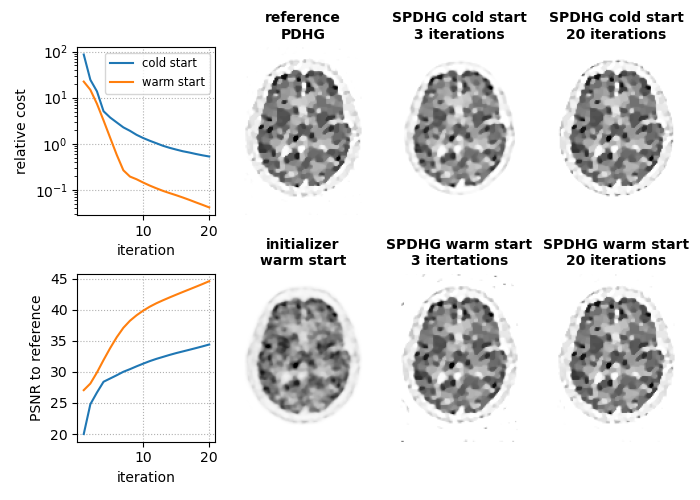
\includegraphics[width=1.0\columnwidth]{figs/SPDHG_cold_vs_warm_start.png}
  \caption{Comparison of convergence of sinogram SPDHG using a cold and warm start
           for 3e5 counts and a TV prior with $\beta = 0.03$ using 112 subsets.
           For the warm start, $x^0$ was taken from 1 EM-TV iteration with 28 subsets
           and $y^0$ was calculated according to \eqref{eq:yinit}.
           Left column: relative cost and PSNR to with respect to the reference solution as
           a function of the iterations.
           Second column: reference PDHG reconstruciton using 20000 iterations (top) and
           initializer $x^0$ used in the warm start.
           Third column: Reconstructions after 3 iterations with cold start (top) and warm
           start start (bottom)
           Fourth column: Reconstructions after 20 iterations.
           Note that in the calculation of the relative cost the same $x^0$ was used
           and that in both cases the same step size ratio $\gamma$ was used.
          }
  \label{fig:warm_start}
\end{figure}


Recalling the fact that more most common TOF PET acquisitions, LM-SPDHG requires less memory and 
is also faster, one would probably prefer LM-SPDHG over SPDHG if the speed of convergence is the same.
In the following we describe a set of numerical experiments that we conducted to show that this
is indeed the case.
This is because in the absence of an analytical solution to the optimization problems \eqref{eq:primal}
and \eqref{eq:saddle}, we analyzed the convergence of LM-SPDHG and SPDHG with respect to a 
reference solution as done in \cite{Ehrhardt2019}.
Convergence was monitored by tracking the relative cost function
\begin{equation}
c_\text{rel}(x) = (c(x) - c(x^*)) / (c(x^0) - c(x^*)) \ ,
\end{equation}
where $c(x)$ is the cost function to be optimized in \eqref{eq:primal} and $x^0$ is the initial value
used for $x$.
Moreover, convergence was also montiored in image space by tracking the peak signal to noise ratio
\begin{equation}
\text{PSNR}(x) = 20\,\log_{10} \left( \|x^*\|_\infty/\sqrt{\text{MSE}(x,x^*)} \right) \ ,
\end{equation}
where $x^*$ is a reference solution obtained by running the deterministic PDHG (SPDHG with only 1 subset)
for 20000 iterations, and MSE is the mean squared error.
Since running PDHG with 20000 iterations using realistic 3D TOF PET data takes a very long 
time (ca. 250\,h), all numerical convergence experiments were performed using simulated 2D TOF PET data.
A 2D software brain phantom with a gray to white matter contrast of 4:1 was created
based on the brainweb phantom \cite{Collins1998} and used to generate simulated 2D TOF data 
including the effects limited spatial resolution, attenuation and a flat contamination mimicking 
random and scattered coincidences with a contamination fraction of 42\%.
The geometry of and TOF resolution of the simulated 2D PET system was chosen to 
mimick one direct plane of the GE SIGNA PET/MR 
(sinogram dimension: 357 radial bins, 224 projection angles, 27 TOF bins, 400\,ps TOF resolution).
Noisy simulated prompt emission TOF sinograms and corresponding listmode data were generated
for different count levels (5e3, 1e6, and 3e6 prompt counts).
Unless stated otherwise, we always used the EM-TV algorithm using 1 iteration and 28 subsets
to initialize $x^0$ and $y^0$ according to \eqref{eq:yinit}.
In all experiments, the step size ratio $\gamma$ was set to $3 / \|x^0\|_\infty$ and $\rho$ was
set to 0.999.
When splitting the data into $n$ subsets, the vector of probabilities determining 
whether an update with respect to a subset of the data of with respect to the prior is 
done was set to 
%
\begin{equation}
p_k = 
  \begin{cases}
  \frac{1}{2n} \ &\text{if } k \leq n \\
  \frac{1}{2}  \ &\text{else} \ ,
  \end{cases}
\end{equation}
%
such that on average an update with respect to the prior was done on every second update
as suggested in \cite{Ehrhardt2019}. 
In this work, we use the term iteration for $2n$ updates such that on average in every iteration
the complete data is forward and backprojected once and $n$ updates with respect to the
prior are performed.

As benchmark examples for non-smooth priors, we consider two ``Total Variation like'' priors
in this work. 
These priors have the form
%
\begin{equation}
  R(Kx) = \|K x\|_{2,1} \ ,
\end{equation}
%
where $\|K x \|_{2,1}$ is the sum over all entries of the pointwise Euclidean norm of $K x$.
The proximal operator for the convex dual of these prior functionals is given by
%
\begin{equation}
(\prox_{R^*}^S(w) )_i = \frac{w_i}{\max(1,|w_i|)} \ .
\end{equation}
%
For the linear operator $K$, we first used discrete forward differences resulting
in the classical Total Variation (TV) prior \cite{Rudin1992}.
Moreover, we also implemented the Directional Total Variation (DTV) prior incorporating
structural information by only considering the component of forward difference operator 
that is perpendicular to a joint gradient field in every point \cite{Ehrhardt2016}.
In our convergence experiments using DTV, we assumed perfect structural prior information
meaning that the joint gradient field used for DTV, was calculated on the ground truth image
itself.
Note that in real acquisitions the quality of the available structural prior information is
never perfect.
However, this should not affect the convergence of SPDHG and LM-SPDHG. 

\subsection*{SPDHG with a warm start vs cold start}

Before investigating the convergene behavior of LM-SPDHG, we first of all tested whether 
a warm start could already help to lead to faster convergence of SPDHG using sinograms.
Figure~\ref{fig:warm_start} shows the results of SPDHG reconstructions with a cold 
($x^0 = 0$ and $y^0 = 0$) and warm start as described above for a data set with 1e6 prompt counts
and a TV prior with $\beta = 0.03$.
It can be seen that the relative cost of SPDHG using the warm start is lower after 8 iterations
and decreases faster compared to SPDHG using the cold start.
Moreover, the PSNR is higher after 4 iterations and increases faster in the early iterations such
that after 20 iterations is closer to there reference PDHG reconstruction.
A similar trend was observed at all count levels, with different $\beta$ values and using
the DTV prior indicating that as expected the warm start helps to accelerate convergence
in the early iterations.
\subsection*{Convergence of LM-SPDHG compared to SPDHG}

Figure~\ref{fig:1e6_TV_003} summarizes the convergence comparison between sinogram SPDHG and LM-SPDHG for
the same data set and prior as described in the previous subsection using the same warm start
for both algorithms.
As demonstrated by the convergence metrics and the reconstructed images, the convergence of
sinogram SPDHG and LM-SPDHG is almost identical.
The same holds smaller and bigger values of $\beta$, different count levels and also the
DTV priors as shown in Fig.~\ref{fig:lm-spdhg-var} and Suppl. Fig. XXX.
For the example with the DTV prior shown in subfigure (c), the convergence in terms of
PSNR seems to be even a bit faster with LM-SPDHG.

\begin{figure*}
  \centering
    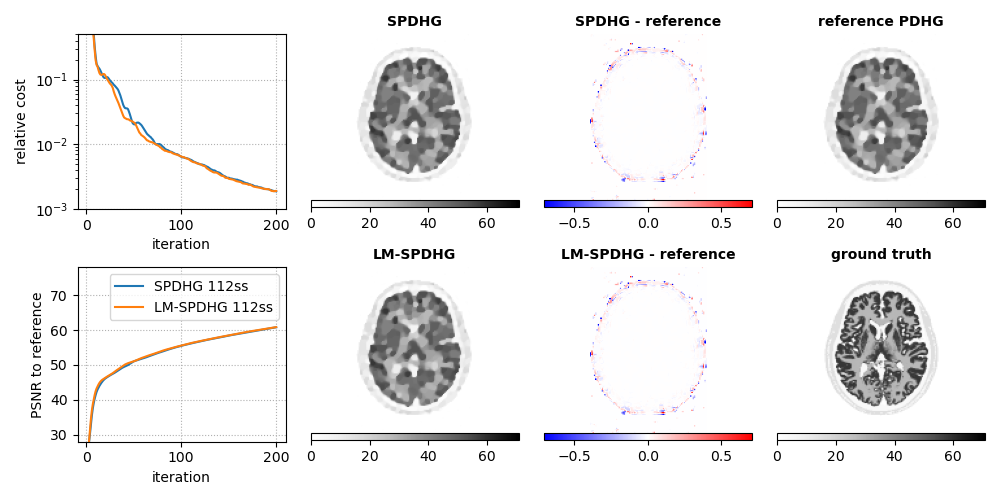
\includegraphics[width=0.8\textwidth]{./figs/brain2d_counts_1.0E+06_seed_1_beta_3.0E-02_prior_TV_niter_ref_20000_fwhm_4.5_4.5_niter_200.png}
  \caption{Comparison of convergence of sinogram SPDHG and LM-SPDHG
           for 1e6 counts and a TV prior with $\beta = 0.03$ using 112 subsets.
           Left column: relative cost and PSNR to with respect to the reference solution as
           a function of the iterations for sinogram SPDHG (blue) and LM-SPDHG (orange).
           Second column: SPDHG (top) and LM-SPDHG (bottom) reconstruction after 200 iterations.
           Third column: absolute difference between SPDHG/LM-SPDHG and reference PDHG reconstruction.
           Forth column: reference PDHG reconstruction using 20000 iterations (top) and ground truth
           used to generate the data (bottom).
          }
  \label{fig:1e6_TV_003}
\end{figure*}


\begin{figure*}
  \centering
  \begin{subfigure}[]{1.0\textwidth}
    \centering
    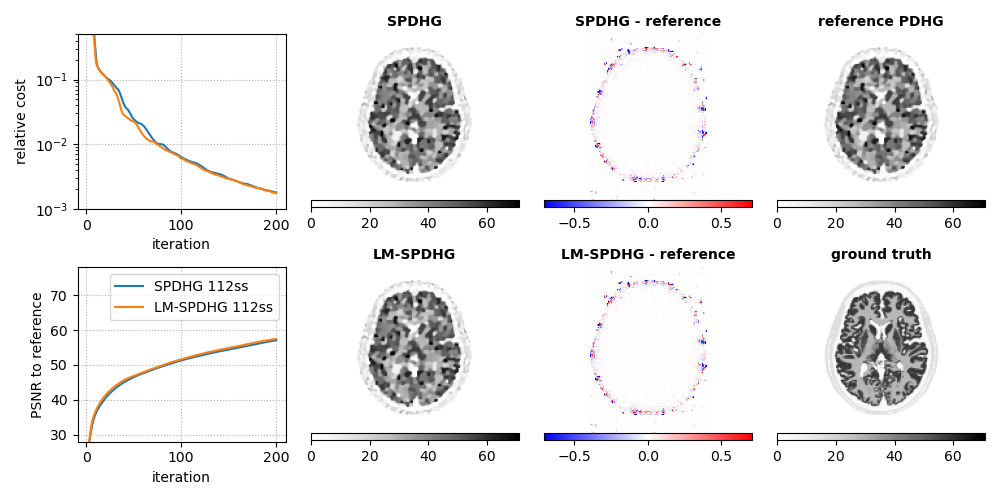
\includegraphics[width=0.8\textwidth]{./figs/brain2d_counts_1.0E+06_seed_1_beta_1.0E-02_prior_TV_niter_ref_20000_fwhm_4.5_4.5_niter_200.png}
    \caption{1e6 counts, TV prior, $\beta = 0.01$}
  \end{subfigure}
  \vfill
  \begin{subfigure}[]{1.0\textwidth}
    \centering
    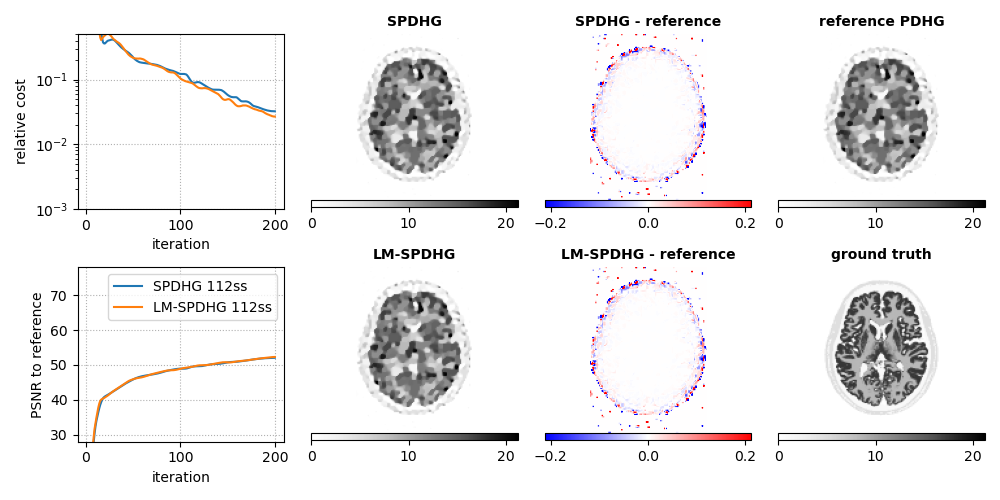
\includegraphics[width=0.8\textwidth]{./figs/brain2d_counts_3.0E+05_seed_1_beta_3.0E-02_prior_TV_niter_ref_20000_fwhm_4.5_4.5_niter_200.png}
    \caption{3e5 counts, TV prior, $\beta = 0.03$}
  \end{subfigure}
  \vfill
  \begin{subfigure}[]{1.0\textwidth}
    \centering
    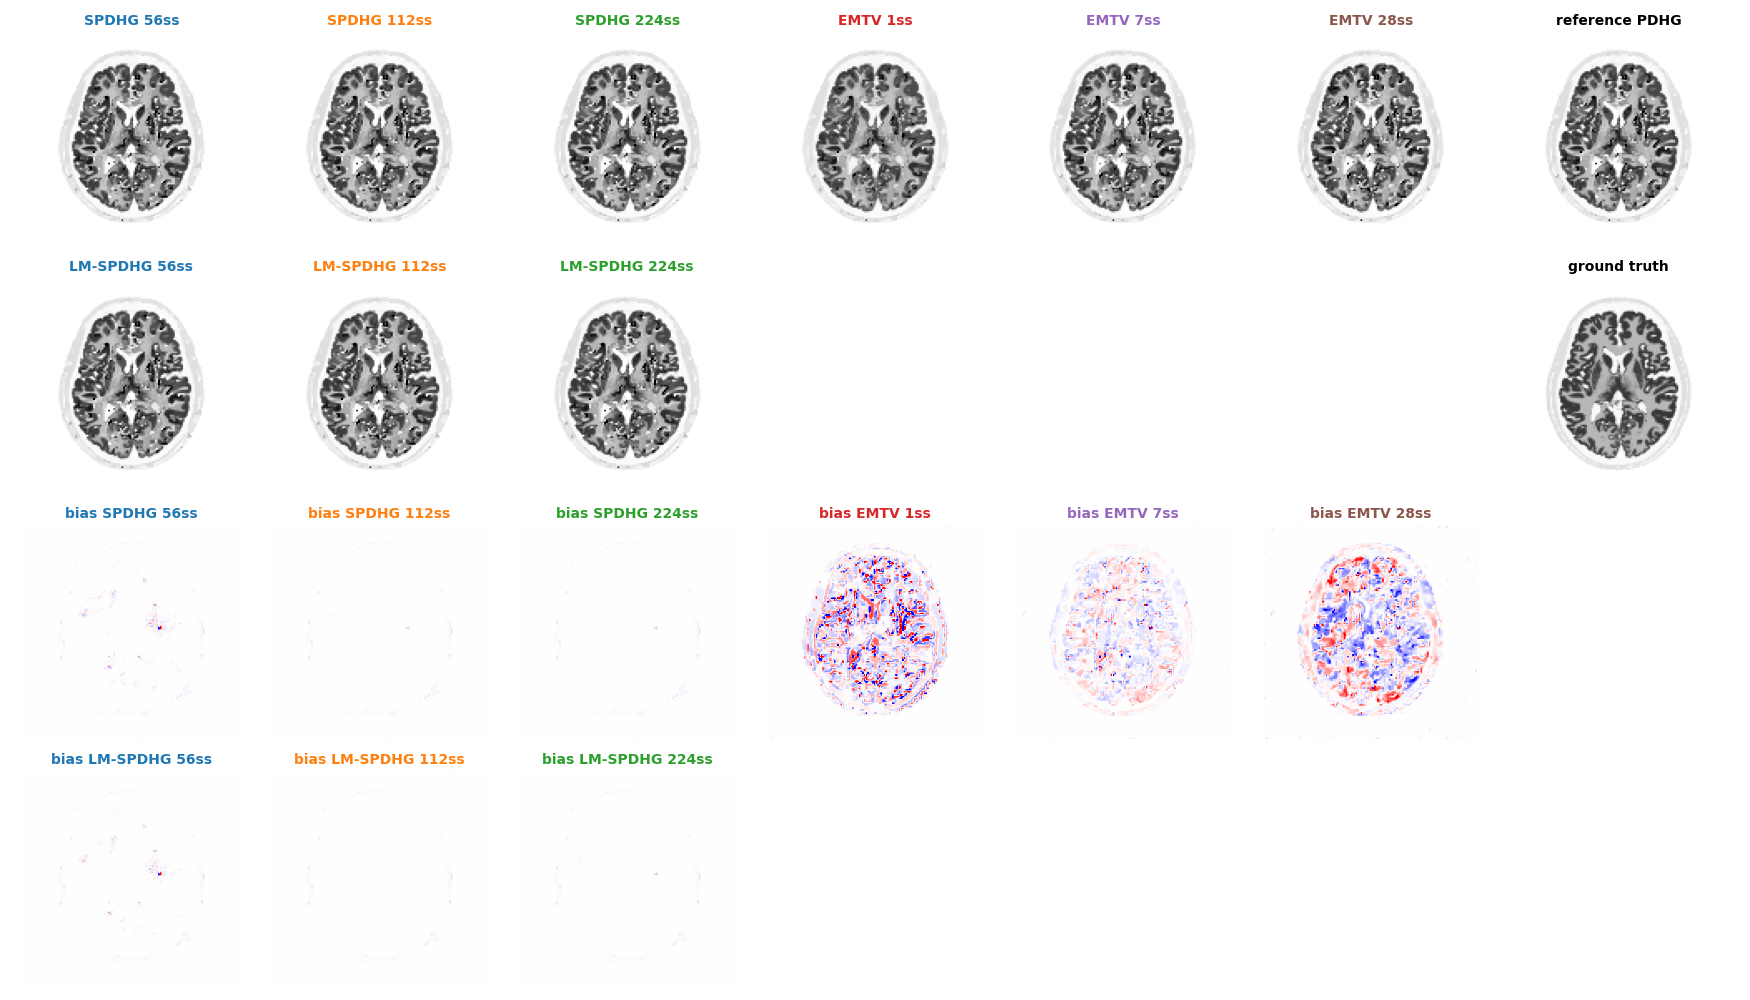
\includegraphics[width=0.8\textwidth]{./figs/brain2d_counts_1.0E+06_seed_1_beta_1.0E-01_prior_DTV_niter_ref_20000_fwhm_4.5_4.5_niter_200.png}
    \caption{1e6 counts, DTV prior, $\beta = 0.1$}
  \end{subfigure}
  \caption{Same as Fig.~\ref{fig:1e6_TV_003} for a smaller value of $\beta$ (a), less counts (b) and the DTV prior (c).}
  \label{fig:lm-spdhg-var}
\end{figure*}




\subsection*{Convergence vs number of subsets}

Figure~\ref{fig:num_subsets} shows the convergence of LM-SPDHG as a function of the number of data
subsets used for low (3e5) and high (3e6) counts and the TV and DTV prior.
It can be seen that in general using 224 subsets leads to faster convergence compared to 56 subsets.
The differences between 56 and 224 subsets are most prominent in the PSNR to refeerence curves 
when using the DTV prior.
For the TV prior - especially at low counts - the differences in terms of PSNR are much smaller
and almost non-existent for the low count example.
For both priors, convergence in terms of PSNR seems slower for 3e5 compared to 3e6 counts.
E.g. in the case of TV, 18 iterations using 224 subsets are needed to reach a PSNR of 40 at 3e5 counts, 
whereas at high counts this threshold is already reached at 3 iterations using 224 subsets.


\begin{figure*}
  \centering
  \begin{subfigure}[b]{0.23\textwidth}
    \centering
    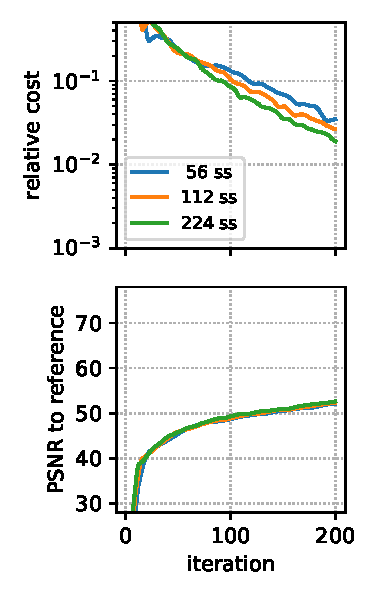
\includegraphics[width=1.0\textwidth]{./figs/brain2d_counts_3.0E+05_seed_1_beta_3.0E-02_prior_TV_niter_ref_20000_fwhm_4.5_4.5_niter_200_ss.pdf}
    \caption{3e5 counts, TV prior, $\beta = 0.03$}
  \end{subfigure}
  \hfill
  \begin{subfigure}[b]{0.23\textwidth}
    \centering
    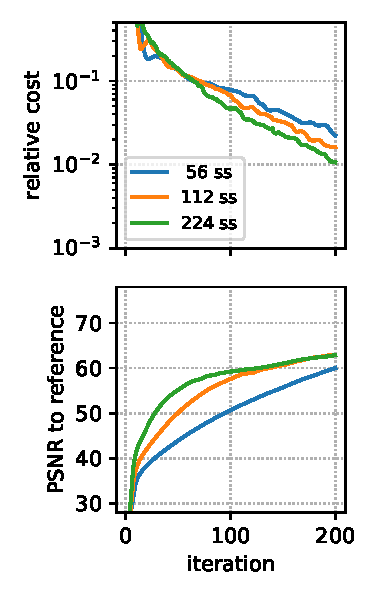
\includegraphics[width=1.0\textwidth]{./figs/brain2d_counts_3.0E+05_seed_1_beta_1.0E-01_prior_DTV_niter_ref_20000_fwhm_4.5_4.5_niter_200_ss.pdf}
    \caption{3e5 counts, DTV prior, $\beta = 0.1$}
  \end{subfigure}
  \hfill
  \begin{subfigure}[b]{0.23\textwidth}
    \centering
    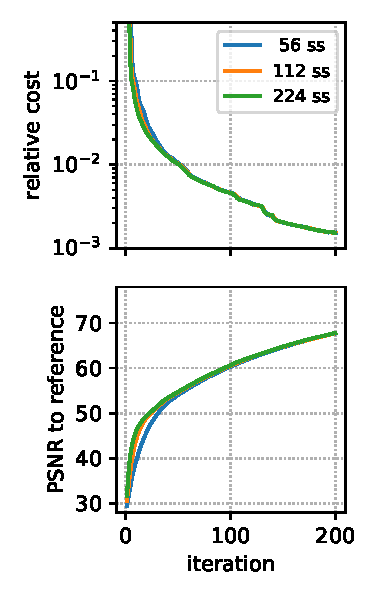
\includegraphics[width=1.0\textwidth]{./figs/brain2d_counts_3.0E+06_seed_1_beta_3.0E-02_prior_TV_niter_ref_20000_fwhm_4.5_4.5_niter_200_ss.pdf}
    \caption{3e6 counts, TV prior, $\beta = 0.03$}
  \end{subfigure}
  \hfill
  \begin{subfigure}[b]{0.23\textwidth}
    \centering
    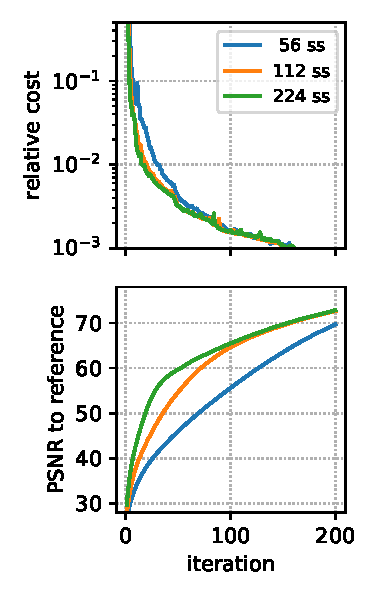
\includegraphics[width=1.0\textwidth]{./figs/brain2d_counts_3.0E+06_seed_1_beta_1.0E-01_prior_DTV_niter_ref_20000_fwhm_4.5_4.5_niter_200_ss.pdf}
    \caption{3e6 counts, DTV prior, $\beta = 0.1$}
  \end{subfigure}

  \caption{Converge of LM-SPDHG for different number of subsets at two count levels for the TV and 
           DTV prior. Note that when increasing the number of data subsets, the number of gradient
           updates per iteration increases as well.}
  \label{fig:num_subsets}
\end{figure*}


\subsection*{3D timing}

% 20cm PET/CT 21 TOF bins: 117s LM, 158s sino per iteration (7e7 counts) 
%                           98s LM, 237s sino per iteration (1e7 counts) 

\section{Discussion}

%\begin{figure*}
%  \centering
%    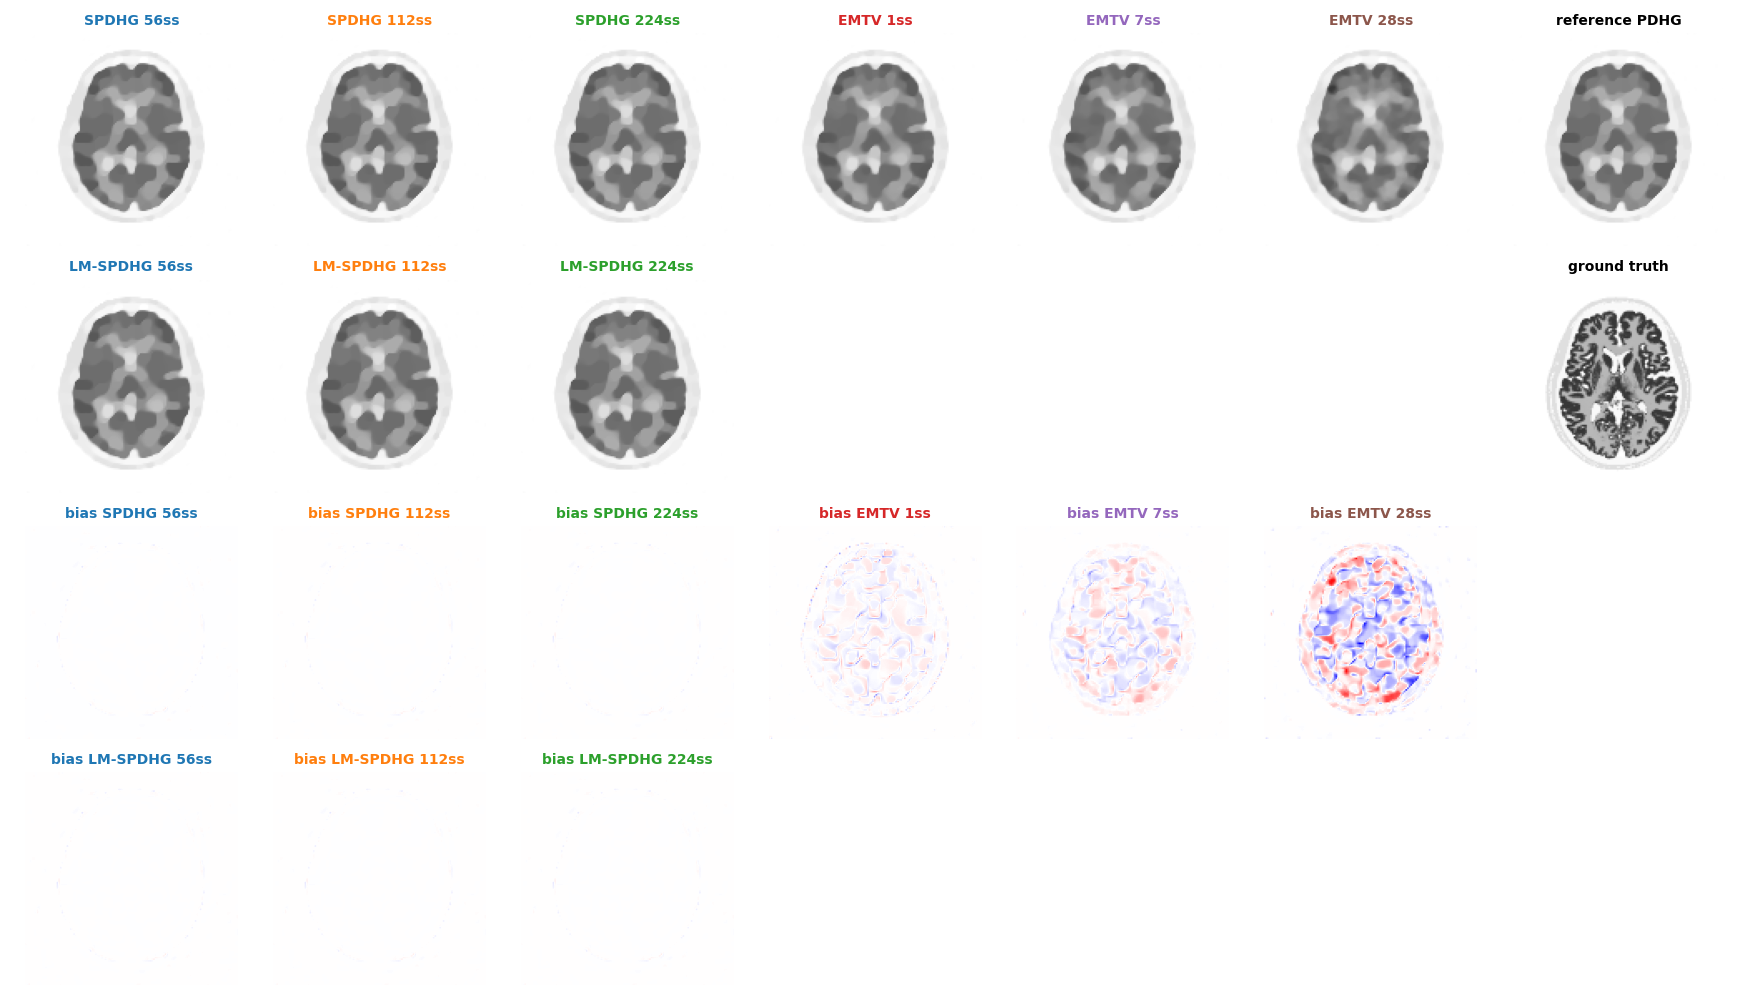
\includegraphics[width=0.8\textwidth]{./figs/brain2d_counts_1.0E+06_seed_1_beta_1.0E-01_prior_TV_niter_ref_20000_fwhm_4.5_4.5_niter_200.png}
%  \caption{$1\cdot10^6$ counts, TV, $\beta = 0.1$}
%\end{figure*}
%
%\begin{figure*}
%  \centering
%    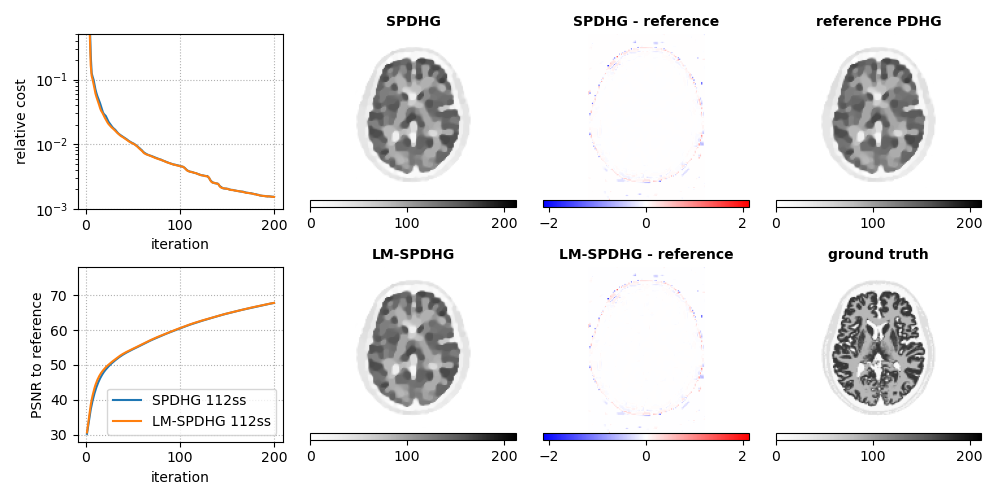
\includegraphics[width=0.8\textwidth]{./figs/brain2d_counts_3.0E+06_seed_1_beta_3.0E-02_prior_TV_niter_ref_20000_fwhm_4.5_4.5_niter_200.png}
%  \caption{$3\cdot10^6$ counts, TV, $\beta = 0.03$}
%\end{figure*}


